\section{User Manual}
\label{usermanual}
The following document is the user manual for the application.


\newpage
\begin{center}
    \vspace*{1cm}
    
    \huge{Gateway 2.0 - User's Manual}
    
    \vspace{2cm}
    \normalsize
    A quick guide for navigating and using \\the Gateway 2.0 application for Android.
    
    
    \vfill
    
    
    \normalsize
    {Rikard Eide\\Andreas Røyrvik\\Jens Kristian Espevik\\Joakim Pettersen\\Magnus Lund\\}
    \vspace{0.8cm}
    NTNU: Norwegian University of Science and Technology\\
    \vspace{0.8cm}
    \today
    \vspace{0.8cm}
    
\end{center}
\newpage

\subsection*{Preface}
This application was designed to be a link between the Vscan application and hospital servers. The application can be started in three different modes; (1) go directly to the "Not yet uploaded"-view, (2) identify the patient and return to Vscan, or (3) start normally with the workflow described in the rest of this guide.

\newpage
\subsection*{Login}
This is the first view you will see when you start the application. From here you can either log into the application or access the settings. To log in to the application, enter your personal username and password and hit the login button. This will start a new session, saving your credentials for up to 10 minutes after the last time you did something in the application. To log out before the 10 minutes has passed, navigate to the "Not yet uploaded" screen and press log out.
If the password you use to log in has changed since the last time the application was started, you will be asked to enter the password you used the last time to change the database password to match the new one.

\begin{figure}[H]
\centering
    \begin{subfigure}[b]{0.49\textwidth}
        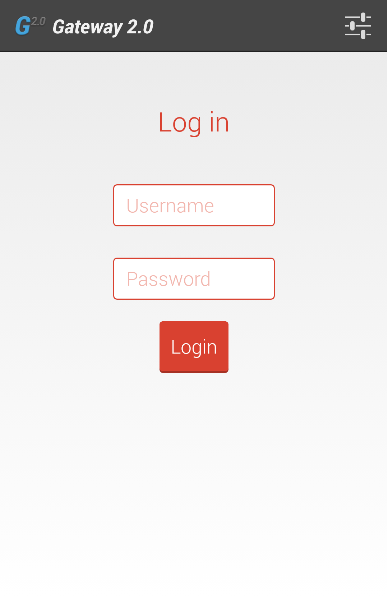
\includegraphics[width=\textwidth]{img/interface/1-Login.png}
        \caption*{Login View}
        \label{fig:01login}
    \end{subfigure}
    \begin{subfigure}[b]{0.49\textwidth}
        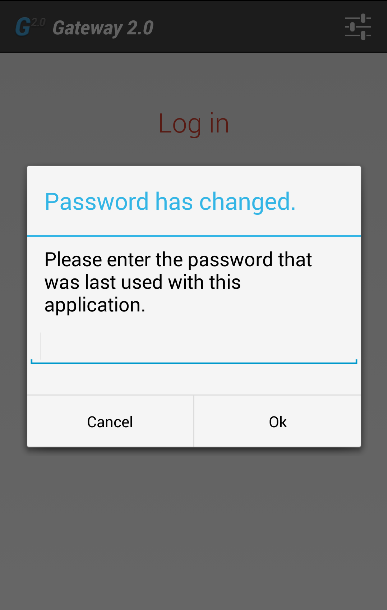
\includegraphics[width=\textwidth]{img/interface/14-DatabasePassword.png}
        \caption*{Password has changed}
        \label{fig:14dbpassword}
    \end{subfigure}
\end{figure}

\newpage
\subsection*{Identify}
In this view you will first have to choose to either identify the patient manually, by typing the SSN, or automatically by scanning a QR code or barcode. To use the automatic feature you will have to install the "Barcode Scanner" application. If you choose automatic mode without having the appropriate application installed, you will be met with a dialog asking you to install it.

When you have chosen the preferred identifying method, you will see a new view with a number input field, where you can enter the SSN or check the SSN gathered from the QR scanner. Pressing the "OK" button will get patient information from the hospital servers and start a new examination.

\begin{figure}[H]
\centering
    \begin{subfigure}[b]{0.49\textwidth}
        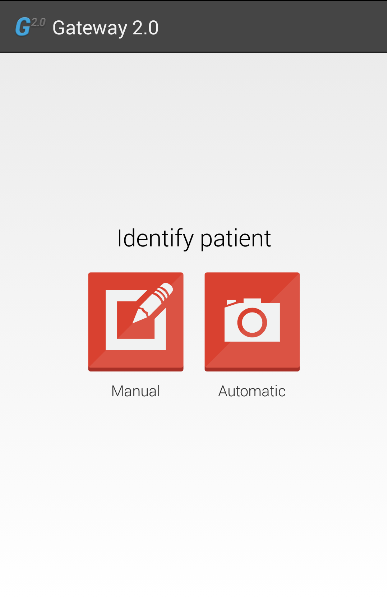
\includegraphics[width=\textwidth]{img/interface/2-Identify1.png}
        \caption*{Choose Identify Method}
        \label{fig:02identify}
    \end{subfigure}
    \begin{subfigure}[b]{0.49\textwidth}
        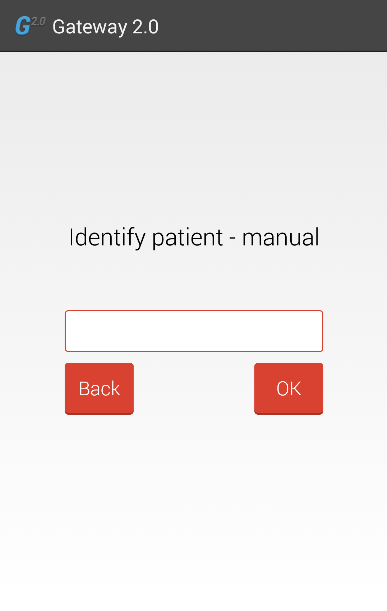
\includegraphics[width=\textwidth]{img/interface/3-Identify2.png}
        \caption*{Enter Patient SSN}
        \label{fig:03identify}
    \end{subfigure}
\end{figure}

\newpage
\subsection*{Examination}
This view will show all available information about the current examination. A small icon next to the SSN will indicate whether the SSN is validated or not. Clicking the SSN, or the small pen icon, will redirect you to the identify view where you can change or validate the SSN. To add an examination comment, click the examination comment text, or the small pen icon in front of it.

Pressing the “View images” button will bring up the commenting view covered in the next section. Two lines of text below the button will tell you the number of images both with and without comment. When you are done with the examination, you can click the “Review and Upload” button, which will bring you to the "Review and Upload" view.

\begin{figure}[H]
\centering
    \begin{subfigure}[b]{0.49\textwidth}
        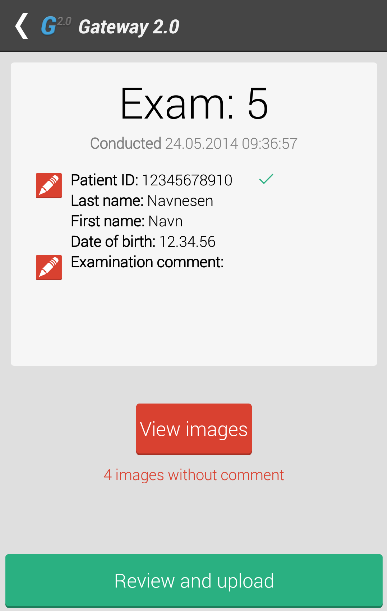
\includegraphics[width=\textwidth]{img/interface/4-Examination.png}
        \caption*{Examination View}
        \label{fig:04examination}
    \end{subfigure}
    \begin{subfigure}[b]{0.49\textwidth}
        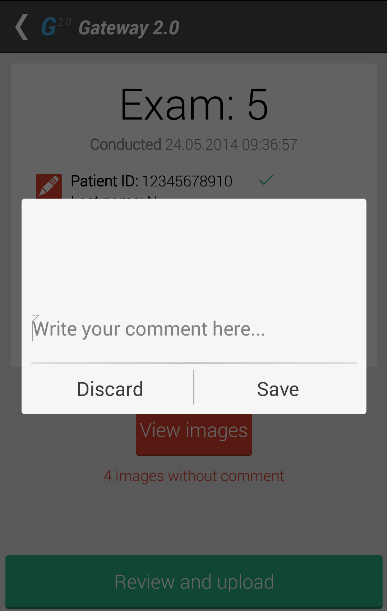
\includegraphics[width=\textwidth]{img/interface/5-ExaminationComment.png}
        \caption*{Examination Comment}
        \label{fig:05examinationcomment}
    \end{subfigure}
\end{figure}

\newpage
\subsection*{Commenting}
In this view you can swipe through all the images in the current examination. At the bottom there are two buttons; the trashcan, which will remove the image from the examination, as well as the commenting button, which will bring up a dialog where you can add a comment to the image. When you are done commenting, you can press the “close” button to return to the "Examination" view. Using the hardware back button will discard all changes and return to the "Examination" view.

\begin{figure}[H]
\centering
    \begin{subfigure}[b]{0.49\textwidth}
        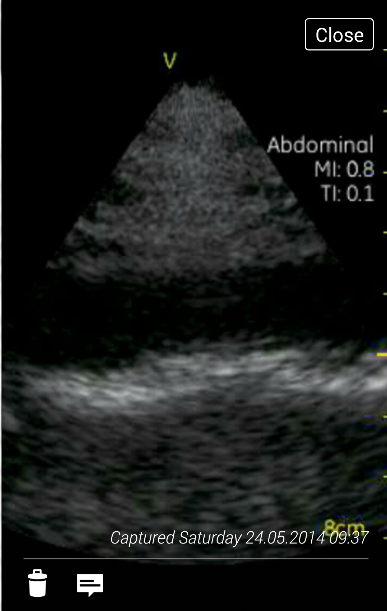
\includegraphics[width=\textwidth]{img/interface/6-ViewImage.png}
        \caption*{Full screen View}
        \label{fig:06viewimage}
    \end{subfigure}
    \begin{subfigure}[b]{0.49\textwidth}
        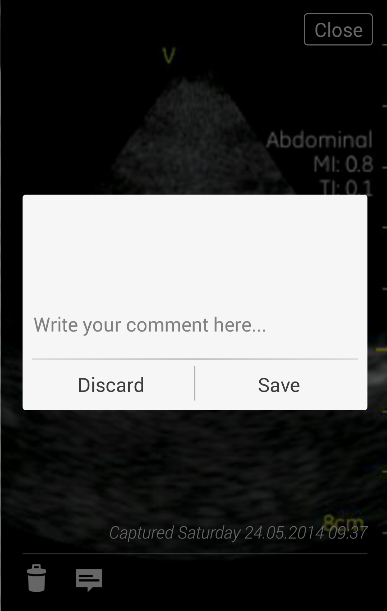
\includegraphics[width=\textwidth]{img/interface/7-ViewImageComment.png}
        \caption*{Enter Image Comment}
        \label{fig:07viewimagecomment}
    \end{subfigure}
\end{figure}

\newpage
\subsection*{Review and Upload}
This view will force you to look through all the information in the examination before uploading it to the hospital servers. When you scroll down to the bottom, there are two buttons: an edit that button will return you to the examination view, and an upload button that will upload the examination. If the upload is successful, the examination will be removed from the local database and you will be redirected to the not yet uploaded view.

If for some reason the upload fails to complete you can press “edit” to go back to the examination view, then the back button to go to the not yet uploaded view. The current examination will remain in the local database, and you can find it in the not yet uploaded view to upload it when you have a connection to the hospital servers.

\begin{figure}[H]
\centering
    \begin{subfigure}[b]{0.49\textwidth}
        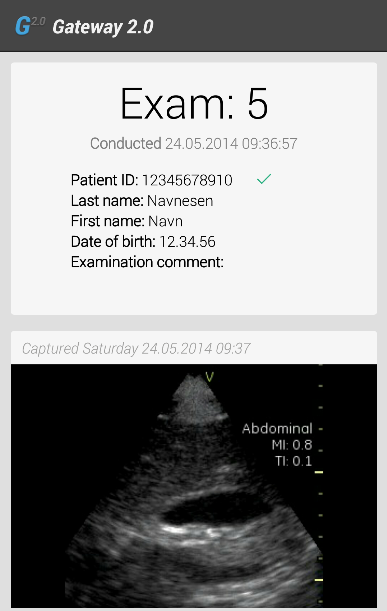
\includegraphics[width=\textwidth]{img/interface/8-ReviewAndUpload.png}
        \caption*{Top of the view}
        \label{fig:08review}
    \end{subfigure}
    \begin{subfigure}[b]{0.49\textwidth}
        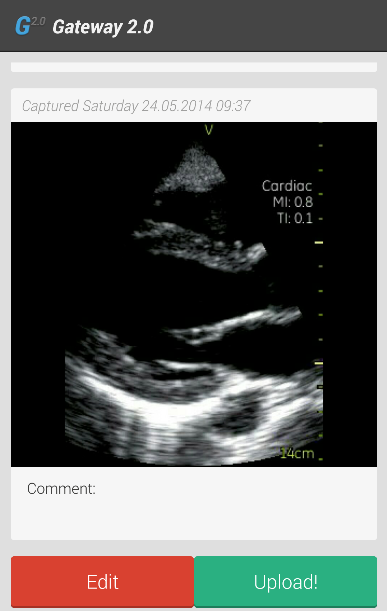
\includegraphics[width=\textwidth]{img/interface/9-ReviewAndUploadEnd.png}
        \caption*{Buttons at the end}
        \label{fig:09reviewend}
    \end{subfigure}
\end{figure}

\newpage
\subsection*{Not yet uploaded}
A list of all saved examinations will be listed in this view. This view is also the only view where you will have the option to log out of the application. Clicking one of the examinations will bring up a dialog where you can choose to either delete the examination from the database or open it in the examination view by choosing edit.

\begin{figure}[H]
\centering
    \begin{subfigure}[b]{0.49\textwidth}
        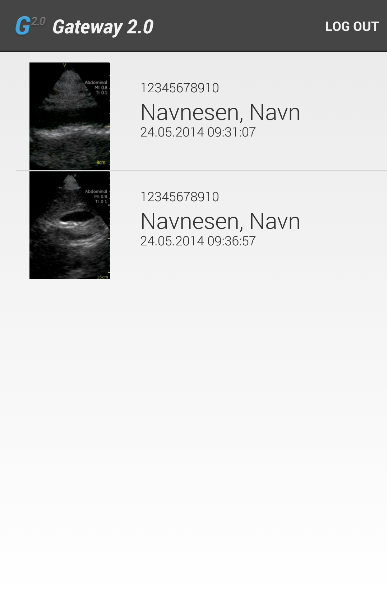
\includegraphics[width=\textwidth]{img/interface/10-NotYetUploaded.png}
        \caption*{Not Yet Uploaded View}
        \label{fig:11notyetuploaded}
    \end{subfigure}
    \begin{subfigure}[b]{0.49\textwidth}
        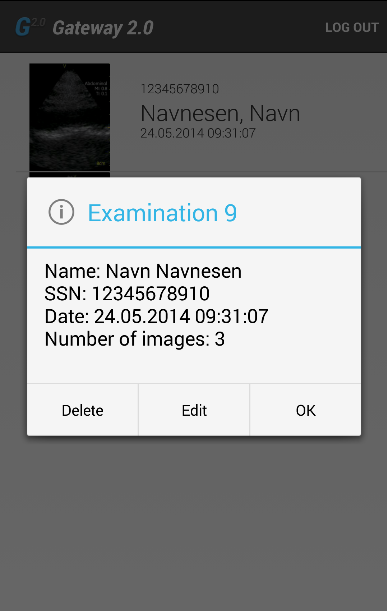
\includegraphics[width=\textwidth]{img/interface/11-DeleteExamination.png}
        \caption*{Examination Choices}
        \label{fig:12delete}
    \end{subfigure}
\end{figure}

\begin{figure}[H]
\centering
    \begin{subfigure}[b]{0.49\textwidth}
        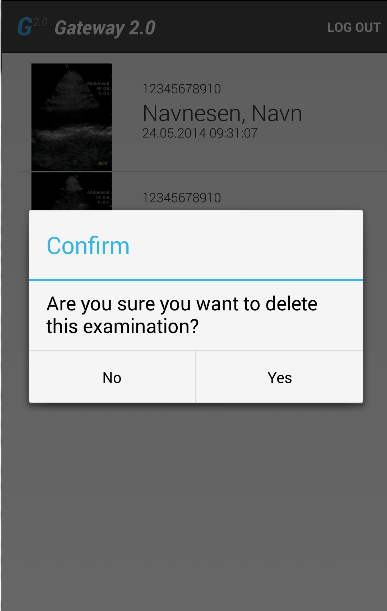
\includegraphics[width=\textwidth]{img/interface/12-ConfirmDeleteExamination.png}
        \caption*{Confirm deletion of examination}
        \label{fig:12confirmdelete}
    \end{subfigure}
    \begin{subfigure}[b]{0.49\textwidth}
        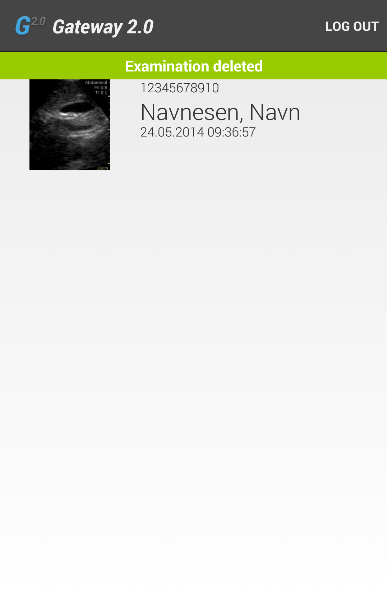
\includegraphics[width=\textwidth]{img/interface/13-NotYetUploadedPostDelete.png}
        \caption*{Not Yet Uploaded view after deletion}
        \label{fig:13notyetuploadedpost}
    \end{subfigure}
\end{figure}

\newpage
\subsection*{Settings}
Then only thing you can do in this view without the technical password is to change the language. More information regarding the other options in this view is explained in the technical manual.

\begin{figure}[H]
\centering
    \begin{subfigure}[b]{0.49\textwidth}
        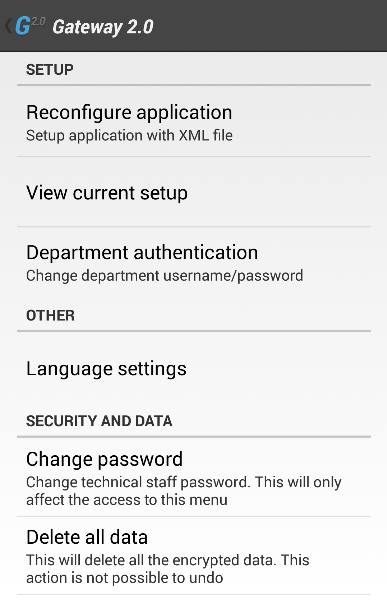
\includegraphics[width=\textwidth]{img/interface/15-Settings.png}
        \caption*{Settings View}
        \label{fig:15settings}
    \end{subfigure}
    \begin{subfigure}[b]{0.49\textwidth}
        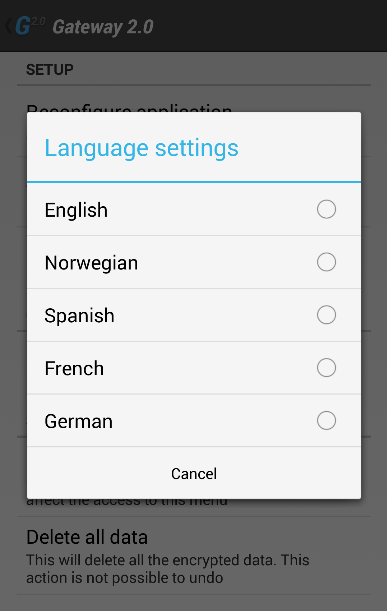
\includegraphics[width=\textwidth]{img/interface/16-Language.png}
        \caption*{Language Select}
        \label{fig:16language}
    \end{subfigure}
\end{figure}

\newpage
\subsection*{Troubleshooting}

\begin{itemize}
\item When the app starts it asks for the tech password.
    \begin{itemize}
	\item The app is not set up properly, contact technical support or refer to the technical manual
	\end{itemize}

\item I have the correct SSN, but the Identify Patient View says it is invalid
    \begin{itemize}
    \item The invalid ID error can be caused by two things; either the entered ID is wrong, or the service is unavailable. Check the SSN one more time, and recheck your network connection.
    \end{itemize}

\item Review and Upload button can not be clicked
    \begin{itemize}
	\item The ID hasn't been validated, click the current ID to validate.
	\end{itemize}
    
\end{itemize}